\documentclass[pdflatex,sn-mathphys-num,lineno]{sn-jnl}

\usepackage{graphicx}
\usepackage{amsmath,amssymb,amsfonts}
\usepackage{amsthm}
\usepackage{booktabs}
\usepackage{xcolor}

\graphicspath{{../../figures/}}
\renewcommand{\arraystretch}{1.12}
\theoremstyle{thmstyleone}
\newtheorem{proposition}{Proposition}
\newtheorem{corollary}{Corollary}
\raggedbottom

\begin{document}

\title[Norm Blind Spot of Amplitude-Encoding Kernels]{The Norm Blind Spot of Amplitude-Encoding Quantum Kernels in Anomaly Detection}

\author*[1]{\fnm{Arnav} \sur{Kapoor}}\email{arnavkapoor23@iiserb.ac.in}

\affil*[1]{\orgdiv{Department of Electrical Engineering and Computer Science}, \orgname{Indian Institute of Science Education and Research Bhopal}, \orgaddress{\city{Bhopal}, \postcode{462066}, \state{Madhya Pradesh}, \country{India}}}

\abstract{Amplitude encoding is a common way to load classical data into quantum kernel
methods. We show that any kernel machine built on it scores an input by a
Rayleigh quotient of a learned matrix. The score depends on the direction of the
input and never on its norm. We ask when this bias helps anomaly detection. We
test it on four security datasets from QKD telemetry and network
flows, with every model trained on the same data at every sample size. In
distribution the amplitude kernel never beats a Gaussian kernel, and it needs more
data when samples are few. On attack types held out from training the outcome
depends on the data. In both simulated settings the kernel fails, because unseen
attacks differ from normal traffic mainly in norm. Appending one constant
amplitude, set to the median training norm, repairs the failure. We explain why
this constant works. Where the norm carries no signal, the anchor can cost
accuracy. On UNSW-NB15 and CIC-IDS2017 the plain kernel does not fail.
@QMI_ABS_ZZ@ @QMI_ABS_SHOTS@ A simple norm statistic does not predict when the
failure occurs. Quantum kernels should be checked for their invariances and tested
on held-out classes from real data, against classical kernels trained at the same
scale.}

\keywords{Quantum kernels, Amplitude encoding, Inductive bias, Anomaly detection, Quantum key distribution, Benchmarking}

\maketitle

\section{Introduction}

Quantum kernel methods map classical inputs to quantum states and use the overlap
of two states as a kernel~\cite{havlicek2019supervised,schuld2021supervised}. Many
quantum models for supervised learning can be written this
way~\cite{schuld2021supervised}. So the question of whether a quantum model helps
often becomes a question about its kernel. Theory says the answer depends on how
the kernel's geometry matches the data~\cite{huang2021power,kubler2021inductive}.
Proven advantages exist only for problems built for the
purpose~\cite{liu2021rigorous}. Benchmarks on standard data rarely find
them~\cite{bowles2024better}.

Security is one of the domains where quantum kernels are now being tried, for
intrusion and botnet
detection~\cite{kalinin2023security,suryotrisongko2022evaluating}. Such studies
face two problems. Circuit simulation is slow, so quantum models are often trained
on a few dozen samples while classical baselines see thousands. Tests also rarely
hold out attack types, although a deployed detector will meet attacks it never
saw~\cite{sommer2010outside}.

This paper studies amplitude encoding, the encoding most often used in that work.
Its kernel can be computed exactly and cheaply on a classical computer. That lets
us remove the first problem. We train it at every sample size on the same data as
classical kernels. We then ask a question that does not need quantum hardware. Is
the inductive bias of this kernel useful for detecting attacks, and when?

The answer turns on one property. An amplitude-encoded state forgets the norm of
its input. We make this exact. Every kernel machine on this kernel scores an input
by a Rayleigh quotient of a learned symmetric matrix
(Proposition~\ref{prop:rayleigh}). The score is blind to the input's norm and to
its sign. Anomaly detectors often rely on exactly this information, since unusual
events tend to lie far from typical data.

We test the consequences in two domains. The first is telemetry from quantum key
distribution (QKD), where implementation
attacks~\cite{huttner1995photon,lydersen2010hacking,gisin2006trojan,bennett1992experimental}
shift channel statistics. The second is network flow monitoring, on a simulator
and on the public UNSW-NB15 and CIC-IDS2017
datasets~\cite{moustafa2015unsw,sharafaldin2018toward}.

Our contributions are as follows.
\begin{enumerate}
\item We show that amplitude-encoding kernel machines compute Rayleigh quotients.
  This gives their exact invariances and their function class.
\item We compare the kernel with classical kernels and other learners at matched
  scale on four datasets.
\item We find that it fails on held-out attack types in both simulated settings,
  and we trace the failure to norm invariance through targeted interventions.
\item We propose a norm anchor that costs one amplitude and at most one qubit. We
  show why the median training norm is a good anchor.
\item We find that the failure does not occur on two public benchmarks, and that
  a simple norm statistic cannot tell the cases apart.
\item We compare an entangling ZZ feature map with tuned bandwidth, and we measure
  the effect of finite-shot kernel estimation.
\end{enumerate}

Section~\ref{sec:related} reviews related work. Section~\ref{sec:theory} derives
the properties of the kernel and the anchor. Section~\ref{sec:protocol} describes
the data and protocol. Section~\ref{sec:results} gives results and
Section~\ref{sec:discussion} discusses them.

\section{Related work}
\label{sec:related}

\textbf{Quantum kernels and their bias.} Havl\'i\v{c}ek et al.\ proposed quantum
feature maps whose kernels may be hard to compute
classically~\cite{havlicek2019supervised}. Schuld showed that many supervised
quantum models are kernel methods~\cite{schuld2021supervised}. Huang et al.\
showed that data can let classical learners match quantum ones, and gave a
geometric test for potential advantage~\cite{huang2021power}. K\"ubler et al.\
argued that quantum kernels need a carefully chosen inductive bias to generalize,
since their feature spaces are very large~\cite{kubler2021inductive}. The encoding
largely sets that bias~\cite{schuld2021effect,larose2020robust}. Our analysis is
an instance of this view, worked out exactly for amplitude encoding.

\textbf{Concentration and bandwidth.} Fidelity kernels on many qubits tend to
concentrate. Off-diagonal entries shrink toward a constant, and exponentially many
shots are then needed to resolve them~\cite{thanasilp2024exponential}. Scaling the
inputs by a bandwidth avoids this and restores
generalization~\cite{shaydulin2022importance,canatar2022bandwidth}. Shot noise
also limits what a kernel can learn on near-term
hardware~\cite{wang2021towards,hubregtsen2022training}. We tune the bandwidth of
our ZZ baseline and simulate finite shots for both quantum kernels.

\textbf{Benchmarking and classical simulation.} Bowles et al.\ found that
out-of-the-box classical models usually beat quantum models on standard
tasks~\cite{bowles2024better}. Tang showed that some proposed quantum speed-ups
vanish against classical algorithms with similar data
access~\cite{tang2019quantum}. Amplitude encoding is classically easy in a
stronger sense. Its kernel has a closed form (Proposition~\ref{prop:exact}). Any
benefit must come from its inductive bias, which is what we measure.

\textbf{Machine learning for QKD and network security.} QKD attacks are countered
by hardware monitoring~\cite{dasilva2012monitoring} and by protocols such as decoy
states~\cite{lo2005decoy} and measurement-device-independent
QKD~\cite{lo2012measurement}. Mao et al.\ detect attacks on continuous-variable QKD
with neural networks~\cite{mao2020detecting}. Machine-learning intrusion detection
is surveyed by Buczak and Guven~\cite{buczak2016survey}. Kitsune popularized
autoencoders trained on benign traffic only~\cite{mirsky2018kitsune}. Quantum
kernels have been applied to intrusion
detection~\cite{kalinin2023security,suryotrisongko2022evaluating} without the
matched-scale and held-out-attack tests we use here.

\section{The amplitude-encoding kernel}
\label{sec:theory}

\subsection{Exact form and cost}

Amplitude encoding pads $\mathbf{x}\in\mathbb{R}^d$ with zeros to $2^q$ entries,
with $q=\lceil\log_2 d\rceil$. It normalizes the result into the $q$-qubit state
$|\psi(\mathbf{x})\rangle=\sum_i \hat{x}_i|i\rangle$, where
$\hat{\mathbf{x}}=\mathbf{x}/\|\mathbf{x}\|$.

\begin{proposition}\label{prop:exact}
The fidelity kernel of amplitude encoding is
\begin{equation}
K_A(\mathbf{x},\mathbf{y}) = |\langle\psi(\mathbf{x})|\psi(\mathbf{y})\rangle|^2
= (\hat{\mathbf{x}}^{\mathsf{T}}\hat{\mathbf{y}})^2 .
\label{eq:ka}
\end{equation}
It costs $\mathcal{O}(d)$ classical operations per pair.
\end{proposition}
\begin{proof}
The amplitudes are real and the padding is zero, so the overlap equals
$\hat{\mathbf{x}}^{\mathsf{T}}\hat{\mathbf{y}}$.
\end{proof}

On hardware, each entry would be estimated by a compute-uncompute or swap-test
circuit. Preparing an arbitrary amplitude-encoded state needs $\mathcal{O}(2^q)$
two-qubit gates~\cite{mottonen2005transformation}. Estimating one entry to
additive error $\epsilon$ needs $\mathcal{O}(1/\epsilon^2)$ shots. A training Gram
matrix on $n$ samples needs $n(n-1)/2$ such estimates. The closed form has none of
these costs. We checked Eq.~\eqref{eq:ka} against a PennyLane
simulation~\cite{bergholm2018pennylane} of the overlap circuit. The two agree to
$7\times10^{-15}$. The simulated circuit takes 26\,ms per entry and the closed form
$3\times10^{-4}$\,ms.

\subsection{The function class}

\begin{proposition}\label{prop:rayleigh}
Let $f(\mathbf{x})=\sum_i a_i K_A(\mathbf{x}_i,\mathbf{x})+b$ be any kernel expansion
on $K_A$, as produced by an SVM, kernel ridge regression or a Gaussian process
mean. Then
\begin{equation}
f(\mathbf{x}) = \hat{\mathbf{x}}^{\mathsf{T}} W \hat{\mathbf{x}} + b,
\qquad W=\sum_i a_i\,\hat{\mathbf{x}}_i\hat{\mathbf{x}}_i^{\mathsf{T}} .
\label{eq:rayleigh}
\end{equation}
So $f-b$ is the Rayleigh quotient of the symmetric matrix $W$ at $\mathbf{x}$.
\end{proposition}
\begin{proof}
$(\hat{\mathbf{x}}_i^{\mathsf{T}}\hat{\mathbf{x}})^2
=\hat{\mathbf{x}}^{\mathsf{T}}\hat{\mathbf{x}}_i\hat{\mathbf{x}}_i^{\mathsf{T}}\hat{\mathbf{x}}$.
Sum over $i$.
\end{proof}

\begin{corollary}\label{cor:inv}
Such a model gives $\mathbf{x}$, $t\mathbf{x}$ and $-t\mathbf{x}$ the same score for
every $t>0$. Its scores lie between $\lambda_{\min}(W)+b$ and
$\lambda_{\max}(W)+b$. Its feature space has dimension $d(d+1)/2$, the space of
symmetric matrices.
\end{corollary}

Proposition~\ref{prop:rayleigh} holds for any training method and any
regularization. We confirmed it numerically for a trained SVM to $10^{-14}$. On
standardized inputs, the origin is the training mean. The norm $\|\mathbf{x}\|$ is
then the distance from typical data. The kernel cannot use it. The corollary makes
a testable prediction. $K_A$ should help when labels depend on direction alone. It
should fail when an attack differs from normal traffic mainly in size.
Figure~\ref{fig:geometry} illustrates the second case.

\begin{figure}[t]
  \centering
  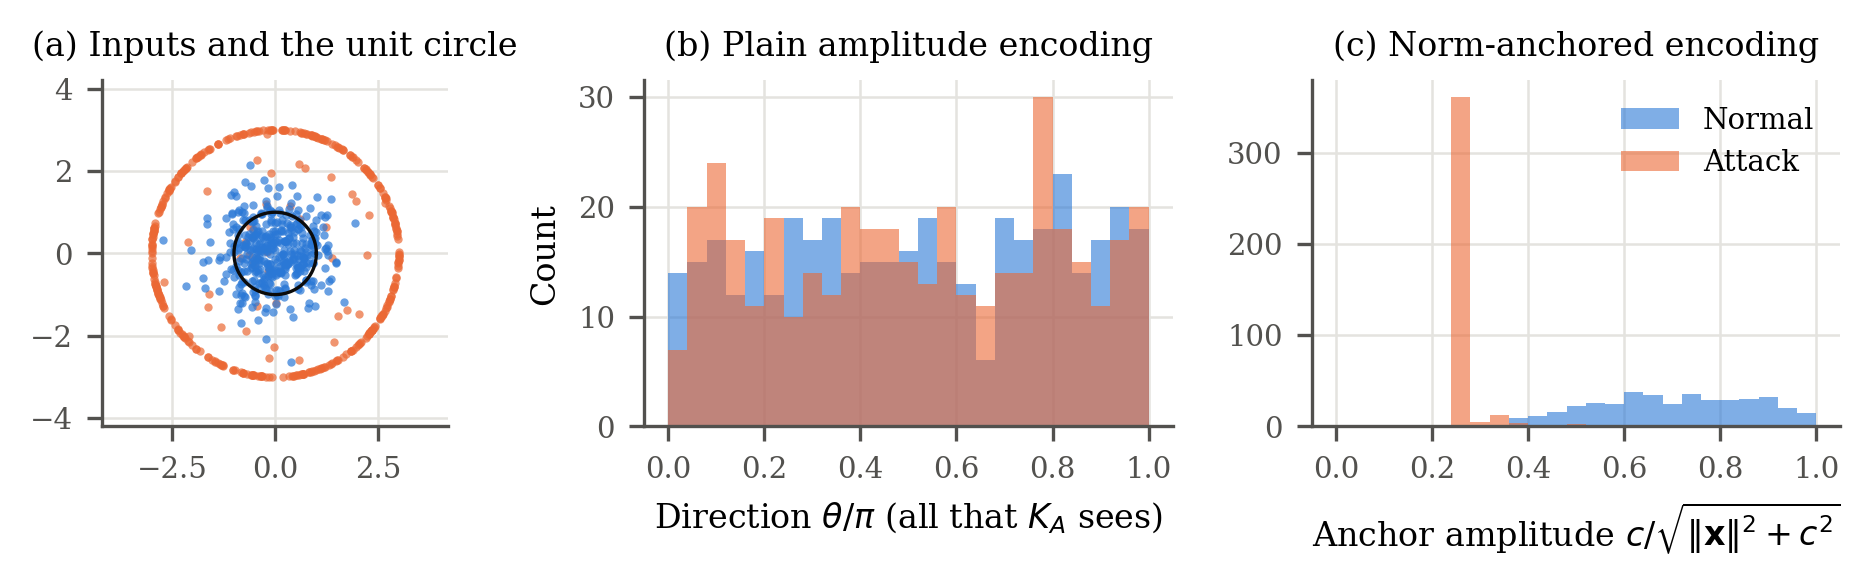
\includegraphics[width=\textwidth]{qmi/fig_geometry.png}
  \caption{Toy data in $\mathbb{R}^2$. Attacks are normal points pushed outward along
  the same directions. (a) Inputs and the unit circle onto which amplitude encoding
  projects them. (b) The direction, the only quantity $K_A$ uses, does not separate
  the classes. (c) The extra amplitude added by the norm anchor separates them.}
  \label{fig:geometry}
\end{figure}

\subsection{The norm anchor}

We append a constant before encoding,
\begin{equation}
\phi_c(\mathbf{x}) = \frac{(\mathbf{x},\,c)}{\sqrt{\|\mathbf{x}\|^2+c^2}},
\qquad c=\operatorname{median}_{\mathrm{train}}\|\mathbf{x}\| .
\label{eq:anchor}
\end{equation}
The anchored kernel is
\begin{equation}
K_c(\mathbf{x},\mathbf{y}) = \frac{(\mathbf{x}^{\mathsf{T}}\mathbf{y}+c^2)^2}
{(\|\mathbf{x}\|^2+c^2)(\|\mathbf{y}\|^2+c^2)} ,
\label{eq:kc}
\end{equation}
a cosine-normalized inhomogeneous quadratic kernel. It needs one more amplitude.
That adds a qubit only when $d$ is a power of two.

\begin{proposition}\label{prop:anchor}
Any kernel expansion on $K_c$ has the form
\begin{equation}
f(\mathbf{x}) = \frac{\mathbf{x}^{\mathsf{T}}A\mathbf{x}+2c\,\mathbf{v}^{\mathsf{T}}\mathbf{x}+c^2 w}
{\|\mathbf{x}\|^2+c^2} + b
\end{equation}
for a symmetric $A$, a vector $\mathbf{v}$ and a scalar $w$. Along a ray
$\mathbf{x}=t\mathbf{u}$ with $\|\mathbf{u}\|=1$, $f$ moves from $w+b$ at $t=0$ to
$\mathbf{u}^{\mathsf{T}}A\mathbf{u}+b$ as $t\to\infty$.
\end{proposition}
\begin{proof}
Apply Proposition~\ref{prop:rayleigh} to $\phi_c(\mathbf{x})$ and split $W$ into
blocks $A$, $\mathbf{v}$ and $w$.
\end{proof}

The anchored model can therefore score by norm. With $A=I$, $\mathbf{v}=0$ and
$w=0$ it computes $t^2/(t^2+c^2)$, which rises with distance from the training
mean. That curve reaches half its range at $t=c$, and its slope peaks at
$t=c/\sqrt{3}$. The model's sensitivity to norm is concentrated around the scale
$c$. If $c$ is much smaller than typical norms, every
input looks far away and norm is invisible again. If $c$ is much larger, every
input looks close to the origin and all states crowd together. The median
training norm puts the steep region where normal data lies, so departures from it
are visible. It uses training data only.

\subsection{Sensitivity}

The Jacobian of $\mathbf{x}\mapsto\hat{\mathbf{x}}$ is
$(I-\hat{\mathbf{x}}\hat{\mathbf{x}}^{\mathsf{T}})/\|\mathbf{x}\|$. Its spectral norm
is exactly $1/\|\mathbf{x}\|$. Normalization shrinks perturbations of large inputs
and magnifies those near the origin. So amplitude encoding gives no uniform
robustness guarantee~\cite{larose2020robust}.

\section{Data and protocol}
\label{sec:protocol}

\begin{table}[t]
  \centering
  \caption{Datasets. Public data uses 20,000 training and 50,000 test flows per
  seed in the main experiments.}
  \label{tab:data}
  \small
  \begin{tabular}{lrrrrr}
    \toprule
    Dataset & Samples & Features & Qubits & Attack types & Seeds \\
    \midrule
    QKD telemetry & 2,000 & 8 & 3 & 4 & 10 \\
    Synthetic flows & 8,000 & 64 & 6 & 5 & 10 \\
    UNSW-NB15 & 257,673 & 68 & 7 & 9 & 5 \\
    CIC-IDS2017 & 2,520,730 & 69 & 7 & 6 & 5 \\
    \bottomrule
  \end{tabular}
\end{table}

\textbf{Testbeds.} Table~\ref{tab:data} lists the four datasets. Each QKD sample is
one key-generation block of a decoy-state BB84 link over 50\,km of
fiber~\cite{lo2005decoy}. Normal operation drifts in loss, detector efficiency,
misalignment, dark counts and background light. Error-rate estimates carry
finite-size noise. Four attacks perturb seven measurements, each scaled by a
strength $s$. We report the hard setting $s=0.3$. Features are the seven
measurements plus a robust Mahalanobis distance to normal
blocks~\cite{rousseeuw1999fast}. The flow simulator draws NetFlow-like marginals
coupled by a Gaussian copula. Five attacks each shift 6 to 7 latent dimensions.
UNSW-NB15 uses its official split. CIC-IDS2017 is cleaned of missing values,
infinite values and 308,381 duplicates. Classes under 100 flows are dropped and
the rest form six families. Public features pass through
$\operatorname{sign}(x)\log(1+|x|)$. All inputs are standardized on training data.

\textbf{Models.} AE-SVM uses $K_A$. AE-SVM (anchored) uses $K_c$. AE-SVM (nonneg)
scales inputs to $[0,1]$ before encoding. This removes the sign ambiguity but keeps
norm invariance. Classical kernels are RBF, Laplacian and cubic polynomial, all in
the same SVM. Above 1,500 samples we use a Nystr\"om
approximation~\cite{williams2001nystrom}. Other models are random forests
(RF)~\cite{breiman2001random}, XGBoost~\cite{chen2016xgboost} and an MLP. On public
data we add a deep network (DNN) and a benign-only
autoencoder~\cite{mirsky2018kitsune}. On QKD data we add a Laplace Gaussian process
(GP)~\cite{rasmussen2006gaussian}, isotonic RF~\cite{zadrozny2002transforming} and
three novelty detectors.

\textbf{Entangling feature map.} To test whether the findings are specific to
amplitude encoding, we add the ZZ feature map of Havl\'i\v{c}ek et
al.~\cite{havlicek2019supervised}. It applies $(U(\mathbf{z})H^{\otimes q})^2$ to
$|0\rangle^{\otimes q}$, with
\begin{equation}
U(\mathbf{z})=\exp\Bigl(i\sum_{j} \beta z_j Z_j
+ i\sum_{j} (\pi-\beta z_j)(\pi-\beta z_{j+1}) Z_jZ_{j+1}\Bigr).
\end{equation}
We use $q=8$ qubits with linear entanglement. Inputs with more than eight features
are reduced by PCA fit on training data, then standardized. The bandwidth $\beta$
is chosen by three-fold cross-validated AUC on the training data, which contains
known attack types only. The candidates are 0.01, 0.02, 0.05, 0.1, 0.2, 0.4 and
0.8. The widths of an
RBF kernel and a Laplacian kernel $\exp(-\gamma\|\mathbf{z}-\mathbf{z}'\|_1)$ are
chosen the same way, with $\gamma q$ set to 0.1, 0.3, 1, 3 or 10. In this experiment all
five kernels see the same eight inputs. Each SVM is trained exactly on 1,000
samples. QKD inputs are used as the QKD pipeline produces them, with the
Mahalanobis distance non-negative. A control setting re-standardizes that column. We simulate the ZZ states exactly. They match
PennyLane to $10^{-15}$.

\textbf{Finite shots.} We model a compute-uncompute estimate of each kernel entry.
An entry with true value $K$ is replaced by $B/S$, where $B\sim\mathrm{Binomial}(S,K)$
and $S$ is the number of shots. Training Gram matrices are kept symmetric with unit
diagonal. Test entries are sampled independently.

\textbf{Protocol.} Every model in a comparison is trained on the same subsample at
every size. Zero-day tests leave one attack type out of training and test on
normal traffic plus that type. We report ROC-AUC there, since it needs no threshold
tuned on known attacks. Intervals are 95\% confidence intervals over seeds. Code
and data preparation are public (see Declarations).

\section{Results}
\label{sec:results}

\subsection{In-distribution detection}

\begin{sidewaystable}
  \centering
  \caption{In-distribution detection (mean $\pm$ 95\% CI over seeds). QKD uses
  $s=0.3$ and $n=1400$. Bold marks the best mean per column. A dash means not run.}
  \label{tab:indist}
  \scriptsize
  \setlength{\tabcolsep}{2.6pt}
  \begin{tabular}{lcccccccc}
    \toprule
    & \multicolumn{2}{c}{QKD telemetry} & \multicolumn{2}{c}{Synthetic flows} & \multicolumn{2}{c}{UNSW-NB15} & \multicolumn{2}{c}{CIC-IDS2017} \\
    \cmidrule(lr){2-3}\cmidrule(lr){4-5}\cmidrule(lr){6-7}\cmidrule(lr){8-9}
    Model & MCC & AUC & Accuracy & AUC & F1 & AUC & F1 & AUC \\
    \midrule
@INDIST_ROWS@
    \bottomrule
  \end{tabular}
\end{sidewaystable}

AE-SVM never beats RBF-SVM in distribution (Table~\ref{tab:indist}). On QKD data
their MCCs are 0.814 and 0.810, and McNemar's test finds no significant seed. On
synthetic flows their accuracies are 0.947 and 0.948 ($p=0.54$). On UNSW-NB15 they
are 0.862 and 0.863 ($p=0.24$). On CIC-IDS2017 RBF-SVM leads by 0.001
($p=0.001$). Tree ensembles are strongest overall. The anchor costs at most 0.003
accuracy on public data. On synthetic flows it helps, reaching 0.960 accuracy
($p<10^{-4}$ against both AE-SVM and RBF-SVM).

Kernel-target alignment~\cite{cristianini2002kernel} is lower for $K_A$ than for
the RBF kernel on every dataset (Table~\ref{tab:align}). This fits
Corollary~\ref{cor:inv}. The amplitude kernel has a small, fixed feature space and
no width to tune.

\begin{table}[t]
  \centering
  \caption{Kernel-target alignment, averaged over attack types.}
  \label{tab:align}
  \small
  \begin{tabular}{lcccc}
    \toprule
    Kernel & QKD & Synthetic & UNSW-NB15 & CIC-IDS2017 \\
    \midrule
@CB_T_ALIGN@
    \bottomrule
  \end{tabular}
\end{table}

\subsection{Sample efficiency}

\begin{figure}[t]
  \centering
  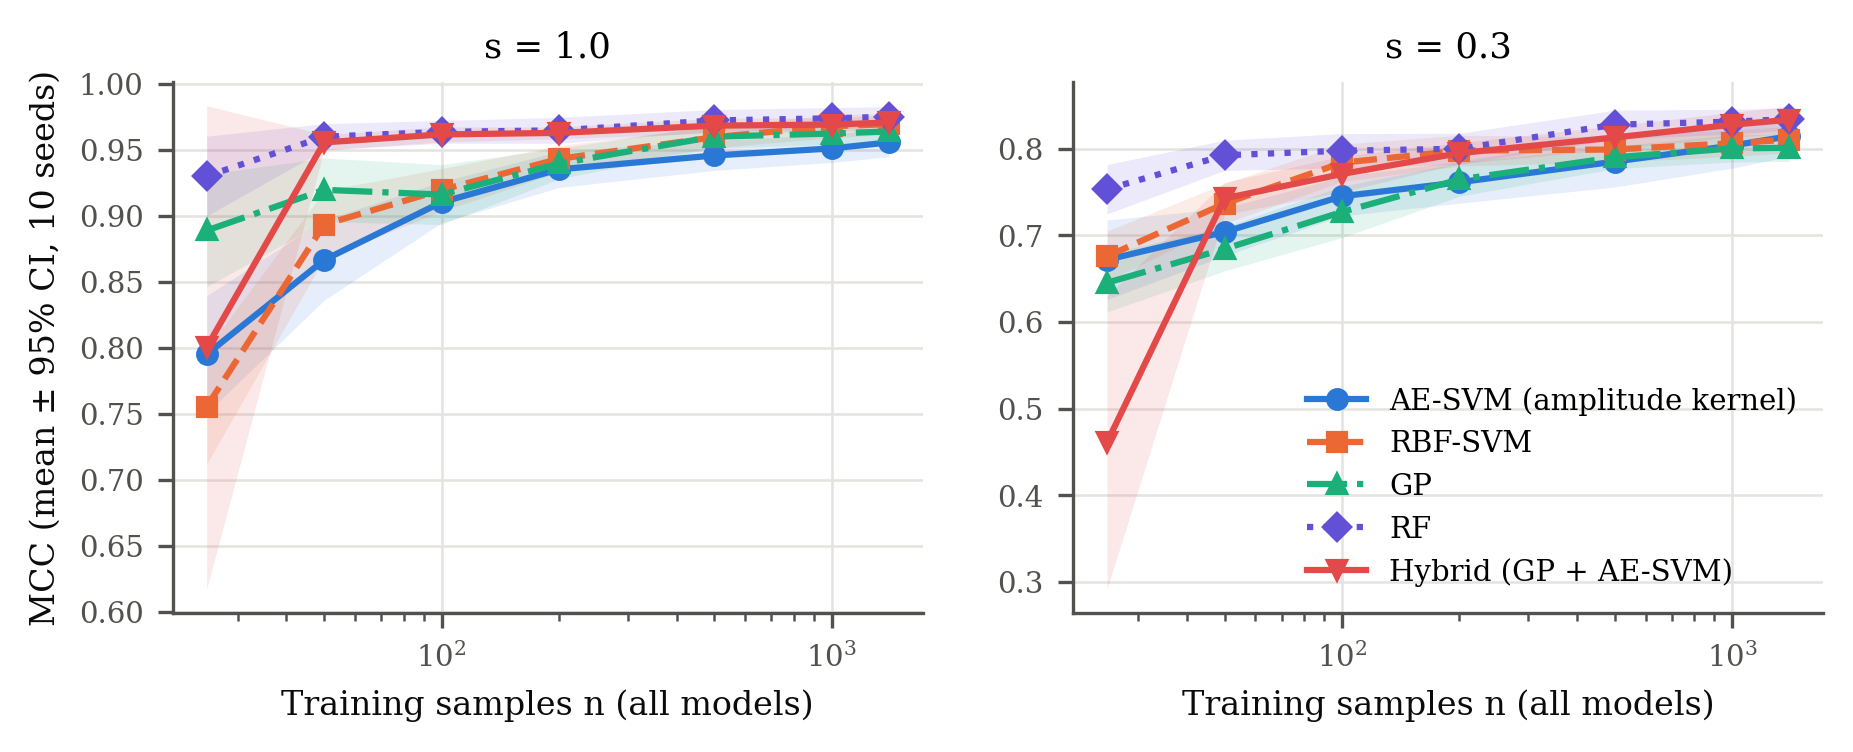
\includegraphics[width=0.95\textwidth]{hyqad/fig3_matched_n.png}\\[4pt]
  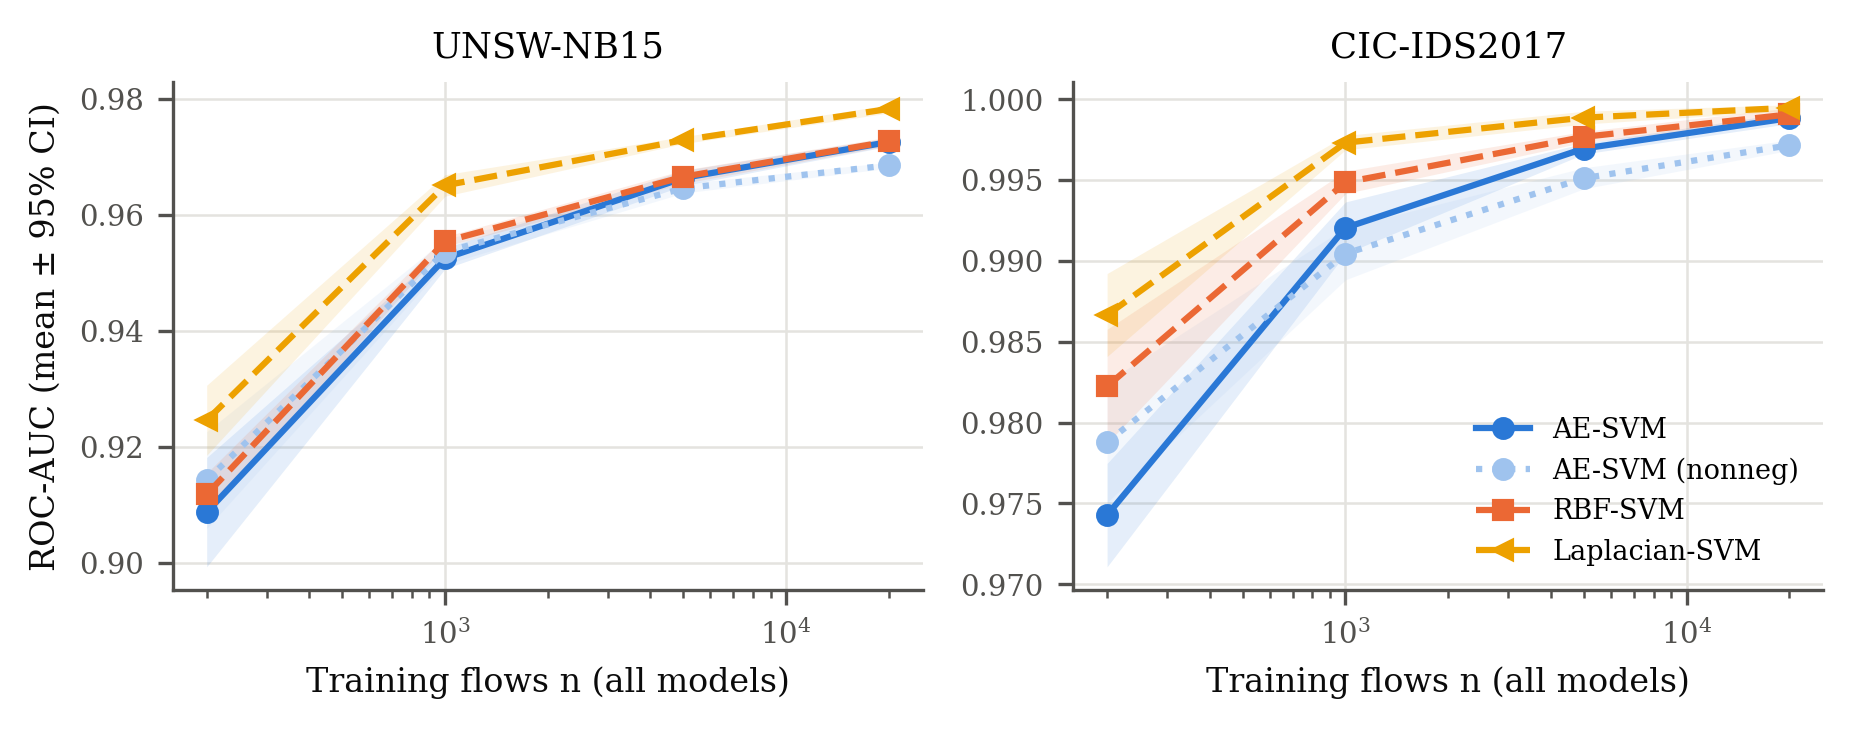
\includegraphics[width=0.95\textwidth]{qztna/fig18_real_matched_n.png}
  \caption{Every model trained on the same subsample at each $n$ (mean $\pm$ 95\%
  CI). Top, QKD telemetry (MCC). Bottom, public data (ROC-AUC).}
  \label{fig:matched}
\end{figure}

Small-sample advantages are a common motivation for quantum kernels. We find none
here (Fig.~\ref{fig:matched}). On QKD data AE-SVM trails RBF-SVM by 0.03 to 0.04
MCC for $n=50$ to 200 and catches up only at $n=1000$. On synthetic flows it trails
by 3.6 points at $n=50$. On CIC-IDS2017 it trails at small $n$. On UNSW-NB15 it
tracks RBF-SVM. The Laplacian kernel is the strongest kernel on public data.

The control tasks of Fig.~\ref{fig:cross} show that the bias can help when it
matches the data. Inputs in $\mathbb{R}^8$ have heavy-tailed norms. When labels
depend on direction only, AE-SVM learns from far fewer samples than any baseline.
When labels depend on norm only, it stays at chance at every $n$, as
Corollary~\ref{cor:inv} requires.

\begin{figure}[t]
  \centering
  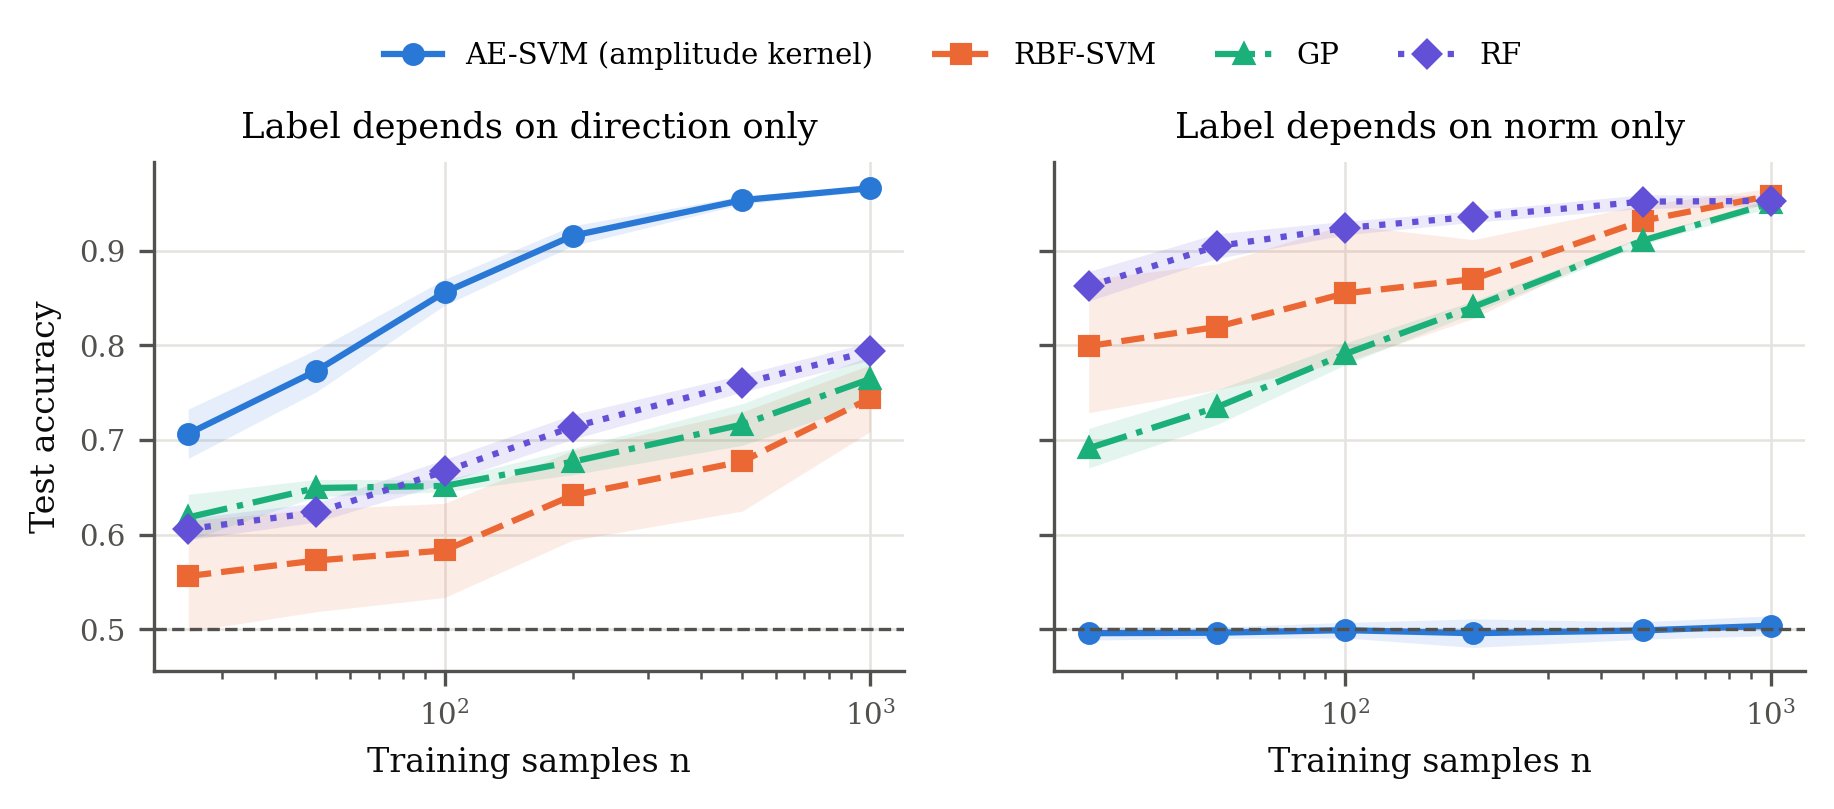
\includegraphics[width=0.9\textwidth]{hyqad/fig8_kernel_crossover.png}
  \caption{Control tasks in $\mathbb{R}^8$ with heavy-tailed norms (mean $\pm$ 95\%
  CI over 10 seeds).}
  \label{fig:cross}
\end{figure}

\subsection{Unseen attack types}

\begin{table}[t]
  \centering
  \caption{Mean ROC-AUC on held-out attack types. QKD uses $s=0.3$. ``No Mahal.''
  removes the only QKD feature that carries magnitude. Bold marks the best per column. A dash means not
  run.}
  \label{tab:zd}
  \small
  \setlength{\tabcolsep}{4pt}
  \begin{tabular}{lccccc}
    \toprule
    Model & QKD & QKD, no Mahal. & Synthetic & UNSW-NB15 & CIC-IDS2017 \\
    \midrule
@CB_T_ZD@
    \bottomrule
  \end{tabular}
\end{table}

\begin{figure}[t]
  \centering
  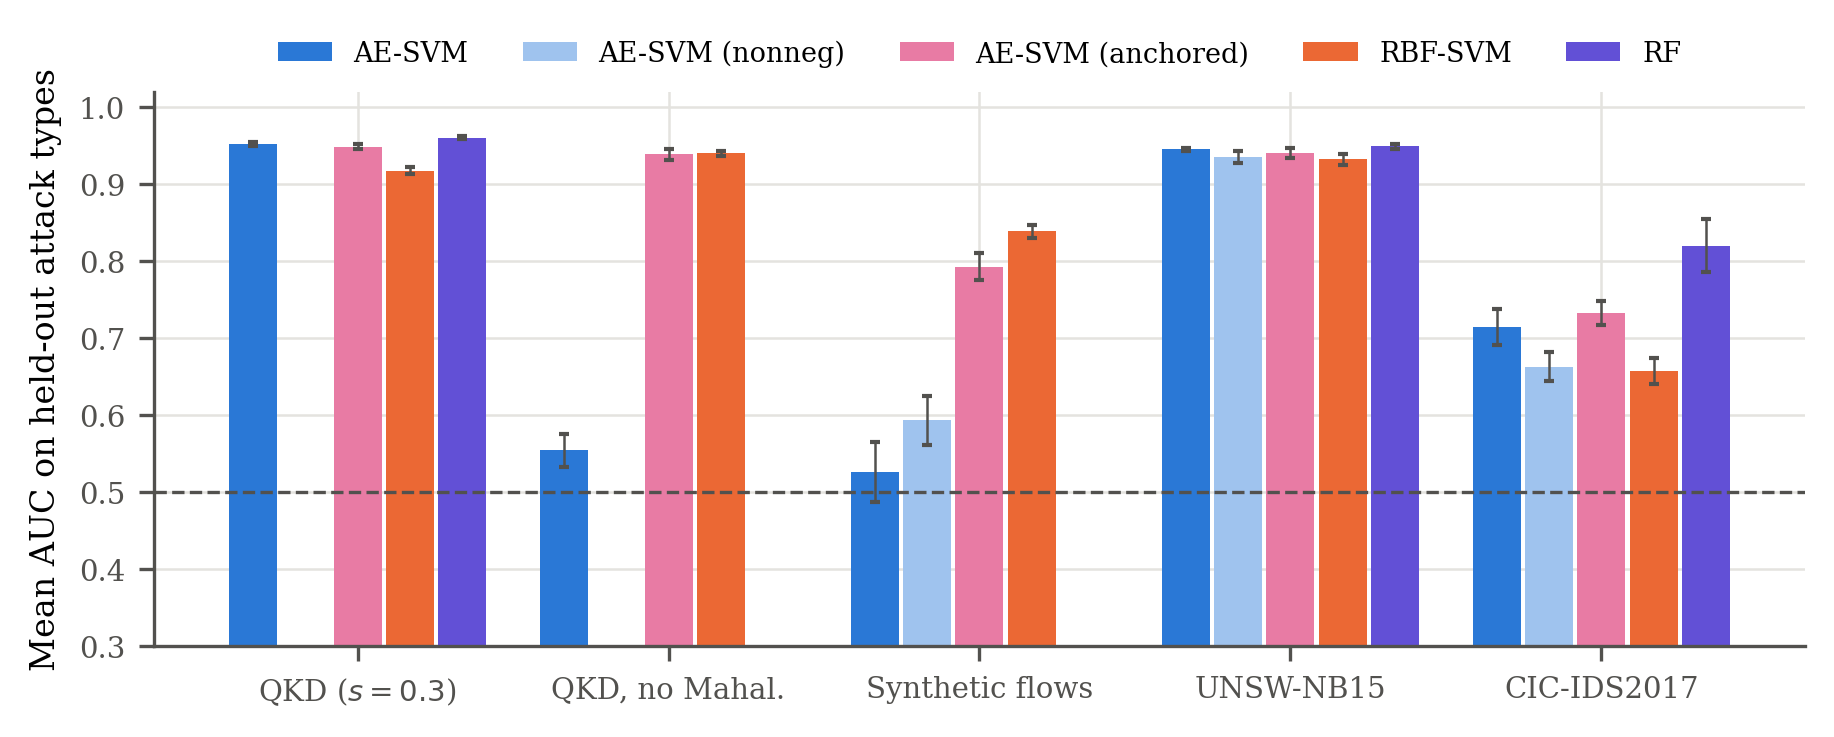
\includegraphics[width=\textwidth]{combined/fig_zeroday_all.png}
  \caption{Mean ROC-AUC on held-out attack types across domains (mean $\pm$ 95\% CI
  over seeds).}
  \label{fig:zeroday}
\end{figure}

Table~\ref{tab:zd} and Fig.~\ref{fig:zeroday} hold the central result. On
synthetic flows plain AE-SVM fails. Every held-out type scores between 0.45 and
0.61, against 0.839 on average for RBF-SVM.

QKD data first looks like a counter-example, since AE-SVM does well there. But one
QKD feature, the Mahalanobis distance, is itself a norm. Removing it drops AE-SVM
to 0.554. RBF-SVM barely changes. With the feature present, the encoding sees the
norm through a coordinate, and the blind spot is covered.

The public benchmarks do not show the failure. AE-SVM matches or beats RBF-SVM on
average. Figure~\ref{fig:perattack} breaks this down by family. On CIC-IDS2017 most
supervised models struggle on Bot and PortScan, and the benign-only autoencoder is
the strongest detector. This matches the closed-world warning of Sommer and
Paxson~\cite{sommer2010outside}.

\begin{figure}[t]
  \centering
  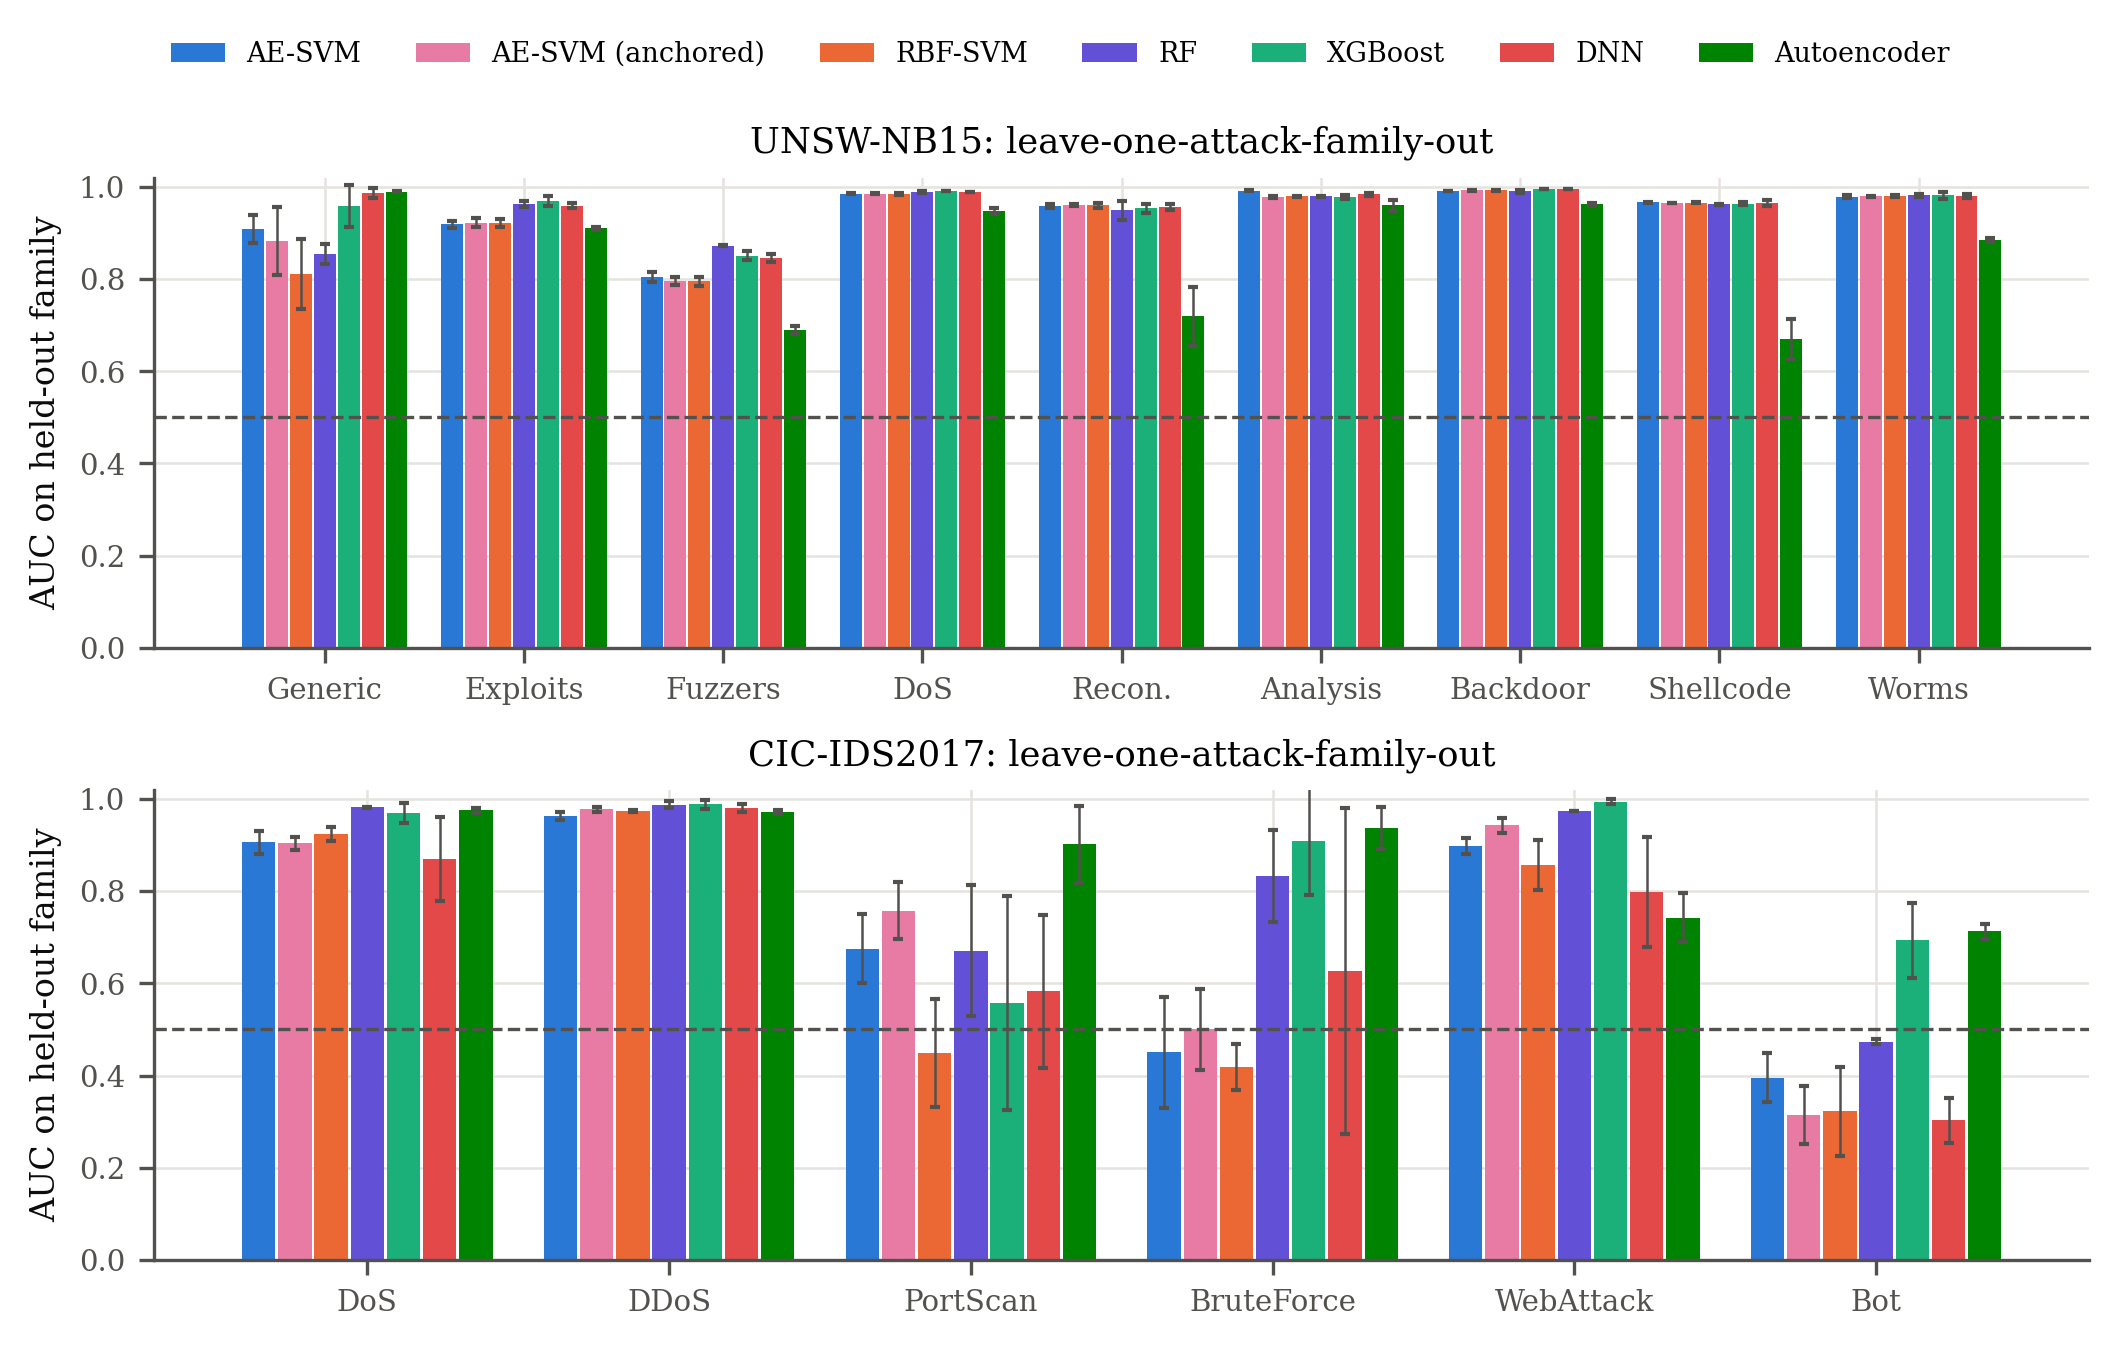
\includegraphics[width=\textwidth]{qztna/fig17_real_zeroday.png}
  \caption{Held-out AUC per attack family on the public benchmarks (mean $\pm$ 95\% CI
  over seeds).}
  \label{fig:perattack}
\end{figure}

\subsection{Mechanism}

Corollary~\ref{cor:inv} offers two causes for the failure, sign ambiguity and norm
invariance. Interventions separate them (Table~\ref{tab:zd}). Scaling to $[0,1]$
removes the sign ambiguity but keeps norm invariance. It helps little on synthetic
flows (0.593). The anchor restores the norm. It closes most of the gap on
synthetic flows (0.793) and all of it on QKD data without the Mahalanobis feature
(0.939). On public data it changes little.

\begin{table}[t]
  \centering
  \caption{Synthetic flows. Mean held-out AUC against the anchor constant $c$
  (5 seeds). $c=0$ is plain encoding. The median rule gives $c\approx6.4$.}
  \label{tab:sweep}
  \small
  \setlength{\tabcolsep}{4pt}
  \begin{tabular}{lcccccccc}
    \toprule
@QZ_T_SWEEP@
    \bottomrule
  \end{tabular}
\end{table}

Table~\ref{tab:sweep} varies $c$. The result follows the shape that
Proposition~\ref{prop:anchor} predicts. Small values leave the norm invisible.
Large values crowd all states together. The median rule lands near the best value
without seeing held-out attacks.

\subsection{An entangling feature map}
\label{sec:zz}

\begin{table}[t]
  \centering
  \caption{Five kernels on the same eight-dimensional inputs, trained exactly on
  $n=1000$ samples (mean $\pm$ 95\% CI over 3 seeds, averaged over held-out types).
  Bold marks the best per row.}
  \label{tab:zz}
  \footnotesize
  \setlength{\tabcolsep}{3pt}
  \begin{tabular}{lccccc}
    \toprule
    Domain & AE & AE (anchored) & ZZ & RBF & Laplacian \\
    \midrule
    \multicolumn{6}{l}{\emph{AUC on unseen samples of known attack types}} \\
@QMI_T_ZZ_IN@
    \midrule
    \multicolumn{6}{l}{\emph{AUC on the held-out attack type}} \\
@QMI_T_ZZ_HELD@
    \bottomrule
  \end{tabular}
\end{table}

\begin{figure}[t]
  \centering
  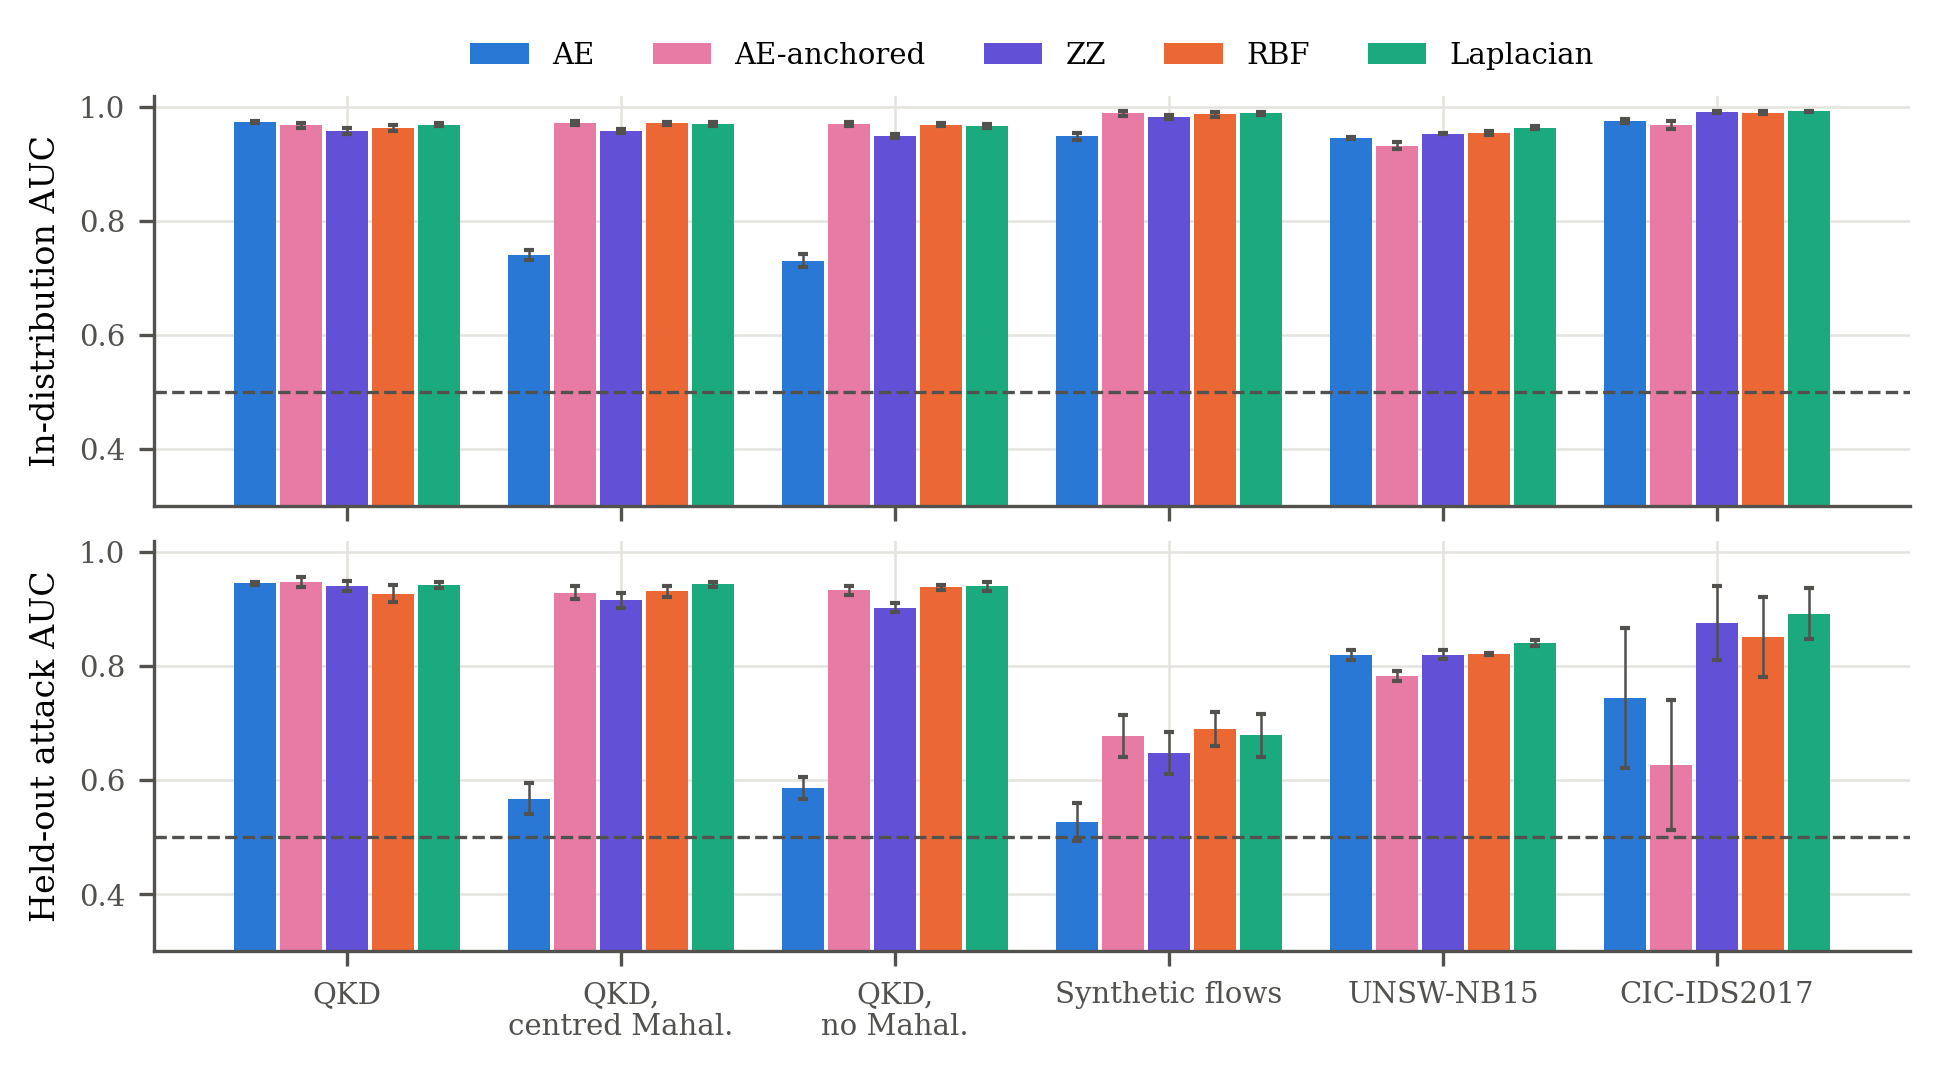
\includegraphics[width=\textwidth]{qmi/fig_feature_maps.png}
  \caption{Kernels on the same eight-dimensional inputs (mean $\pm$ 95\% CI over
  seeds). The ZZ map uses eight qubits and a cross-validated bandwidth.}
  \label{fig:zz}
\end{figure}

@QMI_ZZ_TEXT@

\begin{table}[t]
  \centering
  \caption{Off-diagonal ZZ kernel entries on training data (mean $\pm$ standard
  deviation). For eight qubits a fully concentrated kernel has mean $2^{-8}\approx0.004$.}
  \label{tab:conc}
  \small
  \begin{tabular}{lccc}
    \toprule
    Domain & Selected $\beta$ (median) & Entries at selected $\beta$ & Entries at $\beta=1$ \\
    \midrule
@QMI_T_CONC@
    \bottomrule
  \end{tabular}
\end{table}

@QMI_CONC_TEXT@

\subsection{Finite shots}
\label{sec:shots}

\begin{table}[t]
  \centering
  \caption{Change in mean AUC when every kernel entry is estimated from $S$ shots,
  relative to exact kernels. Averaged over all six settings of Table~\ref{tab:zz}. Training uses
  $n=1000$, which needs about $5\times10^5$ entry estimates.}
  \label{tab:shots}
  \small
  \begin{tabular}{llccc}
    \toprule
    Kernel & Test & $S=100$ & $S=1000$ & $S=10000$ \\
    \midrule
@QMI_T_SHOTS@
    \bottomrule
  \end{tabular}
\end{table}

@QMI_SHOTS_TEXT@

\subsection{Can the failure be predicted?}

\begin{table}[t]
  \centering
  \caption{Norm-versus-direction diagnostic, averaged over held-out attack types. Norm
  AUC scores $\|\mathbf{x}\|$ alone. Direction AUC scores a direction-only distance.
  The last column is AE-SVM minus RBF-SVM held-out AUC.}
  \label{tab:diag}
  \small
  \begin{tabular}{lccc}
    \toprule
    Domain & Norm AUC & Direction AUC & Gap \\
    \midrule
@CB_T_DIAG@
    \bottomrule
  \end{tabular}
\end{table}

A practitioner would like to know in advance whether a dataset falls into the
failure case. We tried the obvious statistic (Table~\ref{tab:diag}). The norm alone
separates attacks best on synthetic flows, where AE-SVM fails. But across held-out
splits it does not predict the gap (@CB_RHO@). It also misses the QKD ablation.
There, removing one coordinate barely changes the norm's separating power yet flips
the outcome. Which features carry magnitude matters more than the norm's overall
power. On real traffic, attack families also differ in which features are active,
and that difference is visible to a direction-only kernel.

\subsection{Calibration and deferral}

\begin{table}[t]
  \centering
  \caption{QKD telemetry, $s=0.3$. Deferral by uncertainty $u=\sqrt{p(1-p)}$.
  Coverage is the share of blocks kept.}
  \label{tab:select}
  \small
  \begin{tabular}{lcccc}
    \toprule
    & \multicolumn{2}{c}{$u<0.3$} & \multicolumn{2}{c}{$u<0.1$} \\
    \cmidrule(lr){2-3}\cmidrule(lr){4-5}
    Model & Coverage & Accuracy & Coverage & Accuracy \\
    \midrule
@HY_T_SELECT@
    \bottomrule
  \end{tabular}
\end{table}

Gaussian-process posteriors are often proposed as a source of uncertainty for
security alerts. On QKD data the Laplace GP is the least calibrated supervised
model, with expected calibration error~\cite{guo2017calibration} $0.047\pm0.006$.
Isotonic RF is the best at 0.030. The GP's probabilities crowd the decision
boundary (Table~\ref{tab:select}). It keeps fewer blocks than isotonic RF or AE-SVM
at the same accuracy, and at $u<0.1$ it keeps none.

\section{Discussion}
\label{sec:discussion}

\textbf{What the encoding decides.} Amplitude encoding fixes a model class before
any training. By Proposition~\ref{prop:rayleigh} that class is the set of Rayleigh
quotients. It contains good detectors only when the label is a function of
direction. This one property accounts for the main pattern in our
results. The bias helps on direction-only control tasks. It hurts when unseen
attacks are mainly larger than normal traffic, as in both simulators. It is
harmless when attack families differ in which features are active, as on both
public benchmarks. The same reasoning applies to any fidelity kernel whose state
preparation normalizes its input. It also applies on hardware, since the
invariance is a property of the state and not of how the overlap is estimated.

\textbf{Simulators can mislead.} Our simulators alone would have suggested that
amplitude encoding is unsafe for zero-day detection in general. The public
benchmarks reversed that. A simple diagnostic did not anticipate which case
applied. We therefore recommend that quantum detectors be judged on held-out
classes from real data, not on simulators alone.

\textbf{Recommendations for quantum-kernel studies.}
\begin{enumerate}
\item Train classical kernels on the same data at every sample size.
\item Derive what the encoding is invariant to before running experiments.
\item If amplitude encoding is used, test the anchored variant on held-out
  classes. The median anchor fixed every failure we saw. On full-dimensional data
  it cost at most 0.005 AUC elsewhere, but on eight-dimensional public data it
  cost more.
\item Tune the bandwidth of angle-encoded kernels and report how concentrated the
  kernel is. Tune classical baselines over grids wide enough that the chosen value
  is not at an edge.
\item Report held-out class results, and for simulated data report single-feature
  separability.
\end{enumerate}

\textbf{Limitations.} QKD attack sizes are modeling assumptions, and to our
knowledge no public QKD attack telemetry exists. The flow simulator is not
packet-level traffic. Both public datasets have known labeling artifacts. We
subsample them to 20,000 training flows, which favours kernel methods. Main
experiment kernels were not tuned per dataset. The ZZ experiment uses PCA to eight
inputs, which removes information that full-dimensional models can use. Its
selected classical widths sat at the top of their grid on public data. We test one
entangling feature map, at one depth and one qubit count. We
simulate shot noise but not gate noise or readout error. Holding out one attack
family only approximates a truly new attack.

\section{Conclusion}

Amplitude-encoding kernel machines compute Rayleigh quotients. They see the
direction of an input and never its norm. At matched scale on four security
datasets this kernel never beats a Gaussian kernel in distribution and needs more
data when samples are few. In both simulated settings it fails on unseen attacks
because it discards the norm. One anchoring amplitude, set to the median training
norm, repairs this, and the theory explains why. On two public benchmarks the
failure does not appear. An eight-qubit ZZ feature map with tuned bandwidth avoids
the blind spot but did not beat tuned classical kernels. Encodings should be chosen and tested for their
invariances, on real held-out classes, against classical kernels at the same scale.

\backmatter

\bmhead{Acknowledgements}
Not applicable.

\section*{Declarations}

\begin{itemize}
\item \textbf{Funding.} No funding was received for this work.
\item \textbf{Competing interests.} The author has no competing interests to declare.
\item \textbf{Ethics approval and consent to participate.} Not applicable.
\item \textbf{Consent for publication.} Not applicable.
\item \textbf{Data availability.} UNSW-NB15 and CIC-IDS2017 are publicly available from
  their original providers. The simulators that generate the QKD and synthetic flow
  data, and all result files, are at \url{https://github.com/arnavk23/quasar-security}.
\item \textbf{Materials availability.} Not applicable.
\item \textbf{Code availability.} All code is at
  \url{https://github.com/arnavk23/quasar-security}.
\item \textbf{Author contributions.} A.K. designed the study, wrote the code, ran the
  experiments and wrote the manuscript.
\end{itemize}

\bibliography{../references}

\end{document}
